\chapter{Register Transfers and the Clock Boundary}

A four-bit shift register is small enough that every possible transition can be checked, yet it poses the problem that every later reconstruction faces. The source machine must be specified, a choice must be made about what counts as an observable step, and a \SP{} history must be shown to reproduce that step. Figure~\ref{fig:mux} gives the rule for selecting an update. Figure~\ref{fig:sr} gives the rule for applying it.

\section{Register Transfers}

A register-transfer description specifies what a machine will store at the next clock edge as a function of its current contents and its inputs. In Figure~\ref{fig:mux}, several sources supply candidate values for $R_0$. The control signals determine which candidate is selected and whether the register loads at all. If every control signal is zero, the register holds its contents. The circuit assumes that at most one source-select signal is asserted. In the prototype, simultaneous assertions therefore produce an explicit control error. That is a choice about how to report a violation of the circuit's assumptions. A priority encoder would give a different machine, with a defined result for some of the same input combinations.

\begin{figure}[ht]
\centering
\begin{tikzpicture}[scale=0.92,font=\small]
 
\draw[thick] (5,0) rectangle (6.6,-5) node[midway]{MUX};
\foreach \y/\l in {-0.8/0,-1.8/{k-1},-3.0/k,-4.2/{n-1}}{
  \draw[bus] (4.6,\y) -- (5,\y) \busmark;
  \node[anchor=west,font=\scriptsize] at (5.03,\y) {$\l$};}
\node at (4.35,-2.35) {$\vdots$};
\node[blk,minimum width=2.8cm] (d0) at (2.0,-0.8) {Dedicated logic $0$};
\node[blk,minimum width=2.8cm] (d1) at (2.0,-1.8) {Dedicated logic $k{-}1$};
\node[blk,minimum width=2.8cm,minimum height=1.4cm] (sh) at (2.0,-3.6) {Registers or\\shared logic};
\draw[bus] (d0.east) -- (4.6,-0.8);
\draw[bus] (d1.east) -- (4.6,-1.8);
\draw[bus] (3.4,-3.0) -- (4.6,-3.0);
\draw[bus] (3.4,-4.2) -- (4.6,-4.2);
 
\node[blk,minimum width=2.5cm] (enc) at (5.8,2.1) {Encoder};
\foreach \x/\l in {5.25/{S_m},5.8/{\cdots},6.35/{S_0}}{
  \node[font=\scriptsize,anchor=west] at (\x,0.85) {$\l$};}
\draw[->,thick] (5.25,1.7) -- (5.25,0);
\draw[->,thick] (6.35,1.7) -- (6.35,0);
 
\node[blk,minimum width=1.7cm,minimum height=1.9cm] (r0) at (9.0,-2.0) {$R_0$};
\draw[bus] (6.6,-2.5) -- (8.15,-2.5) \busmark;
\draw[->,thick] (6.6,-2.5) -- (8.15,-2.5);
 
\node[or gate US,draw,thick,logic gate inputs=nn,scale=0.9,anchor=output] (or) at (9.8,3.7) {};
\node[font=\scriptsize,above] at (or.north) {OR};
 
\draw[thick] (5.2,5.2) -- (5.2,2.6);
\draw[thick] (6.4,5.2) -- (6.4,2.6);
\node at (5.8,4.9) {$\cdots$};
\node[font=\scriptsize,above] at (5.2,5.2) {$K_0$};
\node[font=\scriptsize,above] at (6.4,5.2) {$K_{n-1}$};
\path (5.2,5.2) -- (5.2,2.6) coordinate[pos=0.5] (kk0);
\draw[thick] (5.2,0 |- or.input 1) node[dot]{} -- (or.input 1);
\draw[thick] (6.4,0 |- or.input 2) node[dot]{} -- (or.input 2);
 
\draw[->,thick] (or.output) -- (10.7,3.7) |- (9.0,-0.2) -- (9.0,-1.05);
\node[font=\scriptsize,anchor=south west] at (9.0,-1.05) {Load};
 
\draw[dashed,thick] (9.85,-2.0) -- (11.6,-2.0) -- (11.6,6.0) -- (-0.7,6.0) -- (-0.7,-3.6);
\draw[dashed,thick,->] (-0.7,-0.8) -- (d0.west);
\draw[dashed,thick,->] (-0.7,-3.6) -- (sh.west);
\node[font=\scriptsize,anchor=west] at (11.65,-1.6) {feedback};
\end{tikzpicture}
\caption{Multiplexer selection for $n$ sources. The encoder converts the control lines $K_0,\ldots,K_{n-1}$ into select inputs for the multiplexer, and the OR of the same lines drives the load input of $R_0$. Slashes mark four-bit buses, and the dashed path returns the register contents to the source logic.}
\label{fig:mux}
\end{figure}

In Figure~\ref{fig:sr}, write the four stored bits from left to right as $q=(q_0,q_1,q_2,q_3)$. If the serial input is $b$, then a clock edge gives
\[
(q_0,q_1,q_2,q_3)\;\longmapsto\;(b,q_0,q_1,q_2).
\]
Each stage samples its input from the same pre-edge state. For example, shifting a $0$ into $1011$ leaves $0101$ in the register. The bit shifted out is the old $q_3=1$, and the serial output pin after the edge reflects the new $q_3=1$. Those two observations happen to agree in this example. With $1010$ as the initial word and the same input, the next word is still $0101$, but the bit shifted out is $0$. A prototype that reports a shifted-out bit needs to say which side of the edge it samples.

\begin{figure}[ht]
\centering
\begin{tikzpicture}[scale=0.95,font=\small]
\foreach \i in {0,1,2,3}{
  \draw[thick] (\i*3.0,0) rectangle (\i*3.0+1.7,1.6);
  \node[font=\scriptsize,anchor=west] at (\i*3.0+0.05,1.15) {D};
  \node[font=\scriptsize,anchor=west] at (\i*3.0+0.05,0.4) {C};
  \draw[thick] (\i*3.0,0.15) -- (\i*3.0+0.2,0.4) -- (\i*3.0,0.65);
  \node[font=\scriptsize,anchor=east] at (\i*3.0+1.65,1.15) {Q};
  \node[font=\scriptsize] at (\i*3.0+0.85,1.95) {stage $q_\i$};
  \draw[thick] (\i*3.0-0.45,-0.9) -- (\i*3.0-0.45,0.4) -- (\i*3.0,0.4);
  \node[dot] at (\i*3.0-0.45,-0.9) {};
}
\foreach \i in {0,1,2}{
  \draw[thick,->] (\i*3.0+1.7,1.15) -- (\i*3.0+3.0,1.15);
}
\draw[thick,->] (-1.2,1.15) -- (0,1.15) node[pos=0,left]{SI};
\draw[thick,->] (9.0+1.7,1.15) -- (11.2,1.15) node[right]{SO};
\draw[thick] (-0.8,-0.9) -- (9.4,-0.9) node[right]{Clock};
\end{tikzpicture}
\caption{Four-bit shift register, detailed form. The upper chain carries each bit to the next stage. The lower line reaches all four clock inputs in parallel, so each stage samples its own input at the same edge.}
\label{fig:sr}
\end{figure}

\begin{figure}[ht]
\centering
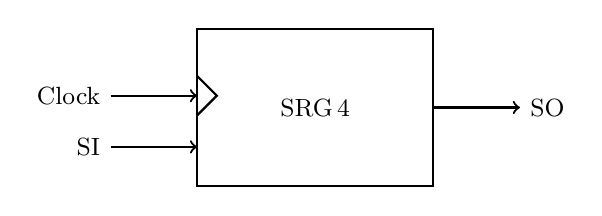
\begin{tikzpicture}[font=\small]
\draw[thick] (0,0) rectangle (3.0,2.0) node[midway]{SRG\,4};
\draw[thick] (0,1.4) -- (0.25,1.15) -- (0,0.9);
\draw[thick,->] (-1.1,1.15) -- (0,1.15) node[pos=0,left]{Clock};
\draw[thick,->] (-1.1,0.5) -- (0,0.5) node[pos=0,left]{SI};
\draw[thick,->] (3.0,1.0) -- (4.1,1.0) node[right]{SO};
\end{tikzpicture}
\caption{Shift-register symbol. The block exposes the same three external connections as the detailed form.}
\label{fig:srg}
\end{figure}

\section{The Boundary in \SP{}}

For a \SP{} reconstruction, the frontier contains four ordered references, one per stage. In the reference kernel the sampled input occurrence is introduced by a $\Bind$ into the open scope and committed at the edge by a $\Pop$, and each destination stage is a $\Bind$ coupled to the occurrence it samples. The four old stage occurrences are popped, because the edge consumes them, and $\Collapse$ publishes the next register word at the clock boundary. The history also retains the old rightmost occurrence, in a separate sphere of kind \texttt{shifted-out}, as evidence of the bit shifted out. This is a proposed encoding for the chapter. Its central implementation requirement is that a reader observing the register at a clock boundary sees a complete word. If an implementation instead reads each stage from a frontier it has already started updating, the new input can propagate farther than one stage in a single simulated edge.

\code{ex_regs_edge}

The faulty variant makes that failure concrete. Each stage reads the frontier that earlier stages have already rewritten.

\code{ex_regs_ripple}

\begin{proposition}[Adequacy at the clock boundary]\label{prop:clock}
For every register word $q\in\{0,1\}^4$ and input $b\in\{0,1\}$, the word published by \texttt{ShiftRegister.edge} equals $(b,q_0,q_1,q_2)$, the sphere of kind \texttt{shifted-out} carries $q_3$, and replaying the recorded history yields the same word and the same shifted-out bit.
\end{proposition}

\begin{proof}
The old word is read once, through a single view, before any event of the edge is committed, so $q$ is fixed. The new stage $k$ is bound with payload $b$ when $k=0$ and with payload $q_{k-1}$ otherwise, both taken from that fixed read. No payload depends on a sphere created during the edge. The \texttt{shifted-out} sphere is bound with payload $q_3$. After the four pops and four binds exactly four stage spheres are live, one per key, so the view sorted by key returns $(b,q_0,q_1,q_2)$. Replay faithfulness (Proposition~\ref{prop:replay}) yields the second claim.
\end{proof}

The first exercise of the book verifies the encoding exhaustively. There are $16$ possible register words and $2$ possible input bits. For each of those $32$ cases the test checks the next word and the old rightmost bit against the equations, then replays the recorded history and checks both observations again. Table~\ref{tab:sr} lists all cases as produced by the prototype.

\begin{table}[ht]
\centering
\begin{tabular}{ccccc}
\toprule
Initial word & Next, input $0$ & Out & Next, input $1$ & Out\\
\midrule
0000 & 0000 & 0 & 1000 & 0 \\
0001 & 0000 & 1 & 1000 & 1 \\
0010 & 0001 & 0 & 1001 & 0 \\
0011 & 0001 & 1 & 1001 & 1 \\
0100 & 0010 & 0 & 1010 & 0 \\
0101 & 0010 & 1 & 1010 & 1 \\
0110 & 0011 & 0 & 1011 & 0 \\
0111 & 0011 & 1 & 1011 & 1 \\
1000 & 0100 & 0 & 1100 & 0 \\
1001 & 0100 & 1 & 1100 & 1 \\
1010 & 0101 & 0 & 1101 & 0 \\
1011 & 0101 & 1 & 1101 & 1 \\
1100 & 0110 & 0 & 1110 & 0 \\
1101 & 0110 & 1 & 1110 & 1 \\
1110 & 0111 & 0 & 1111 & 0 \\
1111 & 0111 & 1 & 1111 & 1 \\
\bottomrule
\end{tabular}

\caption{All thirty-two transitions of the four-bit shift register, generated by the prototype. The column Out is the old $q_3$.}
\label{tab:sr}
\end{table}

Two short counterexamples make clear what those tests protect. The initial state $1000$ with input $0$ must become $0100$, which exposes accidental propagation through multiple stages. The initial states $1010$ and $1011$ with input $0$ both become $0101$, which exposes any attempt to recover the shifted-out bit from the next word alone. The faulty ripple variant above fails the exhaustive test on $28$ of the $32$ cases and turns $1000$ into $0000$, so the test does what it is supposed to do. The ledger distinguishes the $1010$ and $1011$ runs even though their published words are equal, since their chains differ.

\section{Selection as Choice}

The transfer register of Figure~\ref{fig:mux} is the same method applied to selection. Each source supplies a candidate sphere coupled to the current contents of $R_0$. When the control lines select source $k$, the candidate $k$ is popped and every other candidate is refused with the reason \texttt{not-selected}, which is exactly $\Pop(A)\parallel\Refuse(B)$ generalized to $n$ branches. When no control line is asserted the register holds, because the load signal, the OR of the controls, is zero. When more than one control line is asserted the clock is refused: an attempt sphere is bound and refused with the reason \texttt{multiple-select}, an error is raised, and the register is unchanged.

\code{ex_regs_transfer}

With three sources there are eight control combinations. One holds, three select a single source, and four assert more than one line; the test enumerates all eight and checks that the four refused combinations leave the register untouched and are recorded in the ledger.

\transcript{regs}

\section{Why This Chapter Precedes Forth}

That last example gives the Forth chapter a precise starting point. A clock edge and a Forth instruction define different observation boundaries, but both require a rule about what becomes visible when the step completes. The register test checks that the four new stage values come from one old word. The Forth test checks that a word such as \texttt{-} reads its two operands in stack order and publishes one new stack, with enough history to recover the operands that produced it. The shift register lets the reader verify that whole method on a machine whose transition table fits on one page.

\paragraph{Exercise 3.1.} Extend the register to eight bits with a parallel-load control, so that the next word is either the shifted word, a supplied word, or the held word. Decide whether asserting shift and load together is a control error or has a defined priority, and encode the decision as a refusal or a choice accordingly.

\paragraph{Exercise 3.2.} Add a reset that refuses all four stage spheres with the reason \texttt{reset} and binds four zeros. Show that the history still distinguishes a register that was reset from one that was shifted to zero.

\paragraph{Exercise 3.3.} Define the projection that reads the shifted-out bits of the last $m$ edges, and prove that the register word together with those bits determines the word $m$ edges earlier.
